%\documentclass[12pt,a4paper,titlepage]{article}
%\documentclass[12pt]{report}
\documentclass[12pt, a4paper,titlepage]{extreport}
\usepackage[utf8]{inputenc}
\usepackage[english]{babel}
\usepackage{amsmath}
\usepackage{amsfonts}
\usepackage{amssymb}
\usepackage{makeidx}
\usepackage{graphicx}
\usepackage[font=small,labelfont=bf]{caption} % Required for specifying captions to tables and figures
\usepackage{lmodern}
\usepackage{kpfonts}
\usepackage{titling}
% no indent after line break
\setlength\parindent{0pt}
\setlength\parskip{\medskipamount}
%\renewcommand{\familydefault}{\sfdefault}
\usepackage[default]{lato}
\usepackage[T1]{fontenc}
\usepackage{url}
\usepackage{hyperref}

%\usepackage{fontspec}
%\setmainfont[Ligatures=TeX]{Hoefler Text}
%\setsansfont[Scale=MatchLowercase,Ligatures=TeX]{Gill Sans}
%\setmonofont[Scale=MatchLowercase]{Andale Mono}
\usepackage[left=2cm,right=2cm,top=2cm,bottom=2cm]{geometry}
\author{Francesco Gadaleta, PhD}
\date{}
\pretitle{%
  \begin{center}
  \LARGE
  \includegraphics[width=2cm,scale=1,keepaspectratio]{{fitchain_logo_dark_small.png}}\\[\bigskipamount]
}
\posttitle{\end{center}}

\begin{document}

%\begin{figure}[!h]
%   \begin{center}
%     {
\includegraphics[scale=1,width=3cm,keepaspectratio]{fitchain_logo_dark_small.png}}
%    \end{center}
% \end{figure} 
 
\title{\textbf{Amethix - fitchain}\\ The decentralized machine learning factory\\(Technical Primer) }
%\title{fitchain.io\\ The machine learning platform to analyse data \\with confidentiality in mind }

%\author{\textit{Francesco Gadaleta, Ph.D.}}
\maketitle

\begin{abstract}
This paper provides a short introduction to the \textbf{fitchain} platform. 

Fitchain allows data providers to open their private data to algorithms created by data scientists while maintaining secrecy and confidentiality. Three actors are involved in the process of data sharing and model training: \textit{Model Owners} (usually data scientists) who provide the model source code, \textit{data owners} (usually organisations) who provide the data to train models on and \textit{model verifiers} who validate models and maintain consistency about model owners' claims. 
The protocol implemented in fitchain prevents potentially malicious code submitted by \textit{model owners} from tampering with the private infrastructure of \textit{data owners}. In addition, \textbf{fitchain} guarantees that the source code submitted by \textit{model owners} is executed as is. \\
In light of these two essential requirements, the fitchain platform can accommodate the needs of organisations to let their private data be analysed by leveraging a global pool of data scientists who want to provide solutions to the machine learning problems at hand. When security and confidentiality are preserved across the entire process, both data and models become valuable assets that can be traded in the data-model marketplace. A per-project reward and additional incentives are capable of keeping the aforementioned marketplace sustainable and balanced, around what we have identified as a Nash equilibrium \cite{nash}.
\end{abstract}

\section{Introduction}

%\subsection{NOTES}

%What do we want to achieve and why is this important. The benefits of a platform like fitchain.
In the era of machine learning, characterised by effective predictive models, powerful hardware and the capability to collect large amounts of data, both organisations and individuals feel more and more the urge to act on their data in order to extract value about several types of business processes. The progress of machine learning and the success achieved in transforming raw data into knowledge is undeniable \cite{successml}. 

%Democratize data science. Start from data. Now models can be trained only on data that can be accessed. This is not democratic. Demo starts from data. Then models. Data are however an asset and should stay protected. 

Data driven decisions are essential for organisations with complex business dynamics, in which human intervention is usually less effective, often prone to error, and generally speaking much slower than the pace of collecting data. As a matter of fact, data has become a valuable asset, more than ever before. Not only for IT giants like Google, Facebook and Twitter, but also for pharmaceutical and financial corporations it is essential to act on their most valuable asset - data - in order to maintain an advantageous position with their competitors and take decisions faster, minimising losses and maximising profits. As a consequence, the figure of the data scientist has acquired a fundamental role within the settings of many data-driven organisations \cite{forbesds}.

In light of these undeniable facts, no organisation can ignore what we have identified during the years. Data scientists

\begin{itemize}
\item define the quality of the final result of their model
\item prefer to work on challenging problems
\item can not always get access to the data they need
\end{itemize}

Highly skilled data scientists are more likely to design and implement higher predictive models. Hence, hiring the best data scientists in the market can be a game changer for competitive organisations. In addition, initiatives like \textit{Kaggle} \cite{kaggle} are accommodating the fact that highly skilled data scientists prefer challenging problems rather than trivial ones. It is natural for skilled data scientists to constantly change domain, in order to explore new opportunities and put their models to new tests. 
Finally and more importantly, regardless of the domain, it is very difficult to get access to insightful and high quality data, if not after signing non-disclosure agreements (NDAs), or any collaboration contract that preserves secrecy and confidentiality about the data to be shared whenever possible, from a legal perspective.

In contrast, organisations are experiencing other forms of limitation, namely they

\begin{itemize}
\item can not always share their data due to large size or governance restrictions
\item can not keep highly skilled data scientists, who prefer to focus on problems across diverse domains 
\item can not always act on private data that, in turn, keeps getting outdated 
\end{itemize}

The main challenge consists in how can organisations allow data scientists to design their models on data they cannot access, or equivalently how can organisations access a global pool of data scientists without sharing any confidential information with them. 
This is not an easy task for the reasons we identify in the following paragraphs. 

%\paragraph{Data Cleaning}
%Data scientists must see the data they work on, in order to clean it and prepare it for their models to train. Data cleaning is still the most time consuming task of any data analytics pipeline due to the fact that it requires human intervention. Regardless of the advent of very sophisticated artificial intelligence techniques, models are more reliable when trained on clean, high quality data. 

\paragraph{Security}
If data cannot be transferred outside the organisation's infrastructure, then models should be trained at the organisation's site. This clearly opens the door to a plethora of attacks that can be triggered by malicious code, hidden behind a legit machine learning model, tampering with the organisation's infrastructure during model training

\paragraph{Non-repudiation}
Any model that is submitted by a data scientist must be executed \textit{as is}, without the organisation to interfere with the data scientist's implementation and decisions. This requirement usually collides with the security requirement explained in the paragraph above

\paragraph{Traceability}
Any model that has been trained at the organisation's side, must be traced and identified before it is performed within any business context. Moreover, as any other valuable asset, models can be traded and utilised by a community of organisations and other data scientists

We have designed the \textbf{fitchain} platform to accommodate the aforementioned objectives. 


\section{The Fitchain Ecosystem}\label{ecosystem}
Organisations that want to leverage machine learning to extract insight from their private data and extract value for their business, have very few options than undergoing the long hiring process of talented data scientists in a market that is becoming more and more polluted and noisy\cite{forbesds}. 
With fitchain the traditional process of acquiring human resources will dramatically change, allowing organisations to interact with data scientists on a per-project basis. The three actors who operate in the fitchain ecosystem are: data providers, model providers and model validators.

\subsection{The Data Provider}

\begin{center}
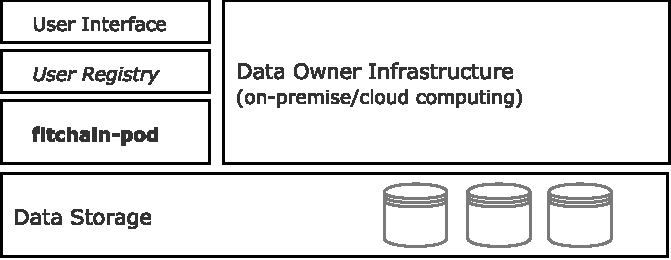
\includegraphics[scale=1]{pod_dataowner.pdf} 
\captionof{figure}{Architecture of the fitchain-pod integrated with the Data Provider's infrastructure. This is the only location where data is available in order to always keep it private. The fitchain-pod is orchestrating requests to use private data from other actors legitimately registered to the User Registry}
\end{center}

The organisation who want a machine learning problem to be solved by performing the best predictive model on private data can connect to the \textbf{fitchain} platform as \emph{Data Provider} and submit a description of the problem to be solved, together with a template of the data required by the data scientist. The aforementioned template is generated by the \textbf{fitchain-pod}, a component that is executed  locally within the organisation's infrastructure. The pod and the entire project are managed via a user friendly interface. 
The data template is \textit{not} the original data and \textbf{does not} contain any sensitive information that would allow anyone to reconstruct the original data source. This is an essential requirement for any organisation to submit their projects publicly and expose only a picture of their data (the original data must remain private).
The owner of the project (eg. the data provider, or any other actor in the fitchain ecosystem) can allocate a project reward that will incentivise data scientists to provide viable solutions for. More specifically, such a reward is the currency that will be used to remunerate the data scientists who provide the best solution, together with the actor who provides the infrastructure for training and the validators who assess the accuracy of the model (as described in the next paragraphs).
Once a model has been submitted, the \textit{fitchain-pod} executed by the data provider, orchestrates and controls the process of model training, during which traces are generated and stored permanently to the available blockchain-based ledger.

\subsection{The Model Provider}

\begin{center}
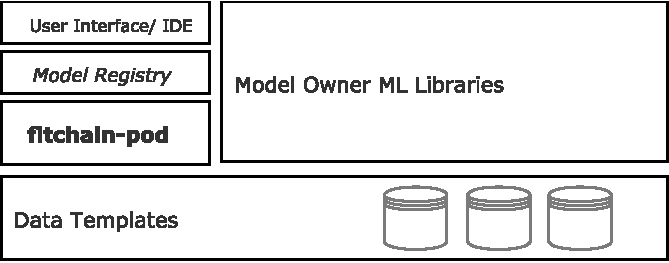
\includegraphics[scale=1]{pod_modelowner.pdf} 
\captionof{figure}{Architecture of the fitchain-pod at the Model Owner's side. This is where the model is implemented with the aid of data template, provided by the data owner's pod. The fitchain pod orchestrates submissions and remote execution of models, tracing them on the Model Registry.}
\end{center}

Data scientists who want to develop a predictive model in the domain of interest can connect to the fitchain platform as \emph{Model Provider}. Such a data scientist might be looking for submitted projects in search for a solution. Needless to say,\emph{Model Provider} will choose the project that is more convenient to her in terms of effort, required skills and offered reward, after which she will start working on a model implementation. This would be possible due to the fact that the project description is supplied with the data template that can be used to assess the compatibility of the model with the original data. A model that \textit{works} on the data template, is supposed to work on the original data too (provided the data owner is not changing the original data without informing her \textit{fitchain-pod}).
Once a model has been implemented and submitted, the pods of the actors involved in the process will orchestrate model deployment and model training within the organisation's infrastructure, the only location where the real (private) data is stored and available. %Needless to say, any attempt to bring the data outside the aforementioned environment will be denied as it violates the security requirements of the \textbf{fitchain pod}.
 
\subsection{The Model Validator}
Any model that is remotely trained, requires to be validated, in order to be deployed in production environments. As a matter of fact, a malicious organisation could train models on fake data, or could fake the entire model training process. 
Model validation is an essential task that is twofold: it discourages organisations to fake model training and assesses the predictive power of models as they become available assets within the fitchain ecosystem.
The model validation process consists of a set of interactions between two actors: \textit{the prover} and \textit{the verifier}. The protocol implemented to validate models by consensus has been designed as an interactive proof system, the details of which are reported in the fitchain whitepaper.
%Validation by consensus Computing consuming mining but in this case the computation which is undeniable serves the purpose.

\paragraph{The prover} is the entity who trained the model and claims its capabilities and metrics (eg. accuracy, error rate, false positive/negative rate, etc.) over the training data. 

\paragraph{The verifier} is the entity who verifies that the aforementioned claims about the model are consistent. Namely, a verifier can create or use validation data of which the response is known, in order to assess the claimed accuracy of the model on such data. 

In order to perform verification, both validation data and model metrics - which together are referred to as \textit{the challenge} - must be accessible at any point in time. Therefore they are stored onto the fitchain public registry. We identified technologies like \cite{oceanprotocol}, BigchainDB \cite{bigchaindb} and IPFS \cite{ipfs} to annotate and trace the validation datasets that are used for model verification.
Technically speaking the challenge-based model verification process is equivalent to the block mining process for blockchains like Bitcoin \cite{bitcoin} and Ethereum \cite{ethereum}.
 
Together with the traces generated by the pod during training, the model verification process constitutes what we refer to as the \textit{proof-of-train}. Needless to say, no sensitive data is stored to the public ledger, nor transferred anywhere else, as the sole purpose of the \textit{proof-of-train} mechanism consists in guaranteeing that organisations and data scientists do not violate the security requirements of the fitchain platform.
%detect suspicious transactions characterising models trained in FIXME (do we have to say this?)


\section{Use Cases}
The fitchain platform has been designed to accommodate the needs of highly regulated environments in which data confidentiality and industrial secrecy must be protected, while giving the opportunity to external actors to interact and use private and protected data. While the most common scenarios would be provided by large organisations who usually own a consistent amount of data and very few resources to analyse them, the \textit{fitchain pod} would also accommodate the needs of individuals who can monetise their data by allowing other actors to use it without accessing or ever own it. 

We hereby describe some of the most interesting yet common use cases in which the fitchain platform would express its potential fully.

% Transportation Uber is now using Machine Learning technology to more efficiently allocate its cars and drivers, seeking to ensure riders can always get a ride when they need one, without having to pay surge pricing.

%Robotics Using complex Machine Learning algorithms—and a range of sensors and motion capture cameras that feed data to the algorithms—computer scientists at The University of Washington have built a robotic hand that can actually “learn” to get better at its tasks.

%Entertainment First, Machine Learning started predicting the movies we want to watch (Netflix). Now, it's creating the movies! A collaboration between a filmmaker and a data scientist has produced a film written entirely by a recurrent neural network named "Benjamin."

% Security Finance companies like PayPal are using deep learning techniques to analyze gargantuan amounts of data in the service of preventing fraud, and companies are using increasingly sophisticated behavioral analytics tools to prevent security breaches.


\subsection{Healthcare\&Pharma}
Pharmaceutical companies represent one of the most regulated environments in data science. Pharmacological and medical data, chemical compounds for drug discovery, medical claims, and sales statistics of drugs in their portfolio, represent only a tiny fraction of the amount of data that such organisations usually deal with. 
Acting on such data via machine learning and predictive analytics is one powerful strategy that many organisations have already experienced and cannot deny the benefits of. Entire organisations have been restructured to weaponise themselves with teams of data scientists in order to extract the hidden knowledge from their data, otherwise sitting in their infrastructure, becoming obsolete and more expensive to store. 
The pool of available data scientists however is not unlimited and the scarcity of such skilled individuals has led the very same organisations to deal with external contractors, or to hire the data experts the local market had to offer. 
Fitchain can change this, by improving the way pharmaceutical organisations will interact with their collaborators, globally spread, without any constraint. Bridging the gap between private data and data scientists on a global scale is a fundamental step that allows large and small healthcare organisations to access data experts that otherwise could have never been accessed, in turn, providing the best solutions to the problems submitted via the platform. 
Moreover, data can be consumed wherever it is created, without the necessity to be moved across cloud storage facilities, cancelling the risks of leakage and loss, a very strict requirement for organisations operating with sensitive medical data. Fitchain brings computing to the data, facilitating the transfer of the trained models from their owners to their direct users.  
%Using deep learning and artificial intelligence, a new microscope can capture and analyze cell images at a rate of 36,000/second, allowing it to locate cancer cells with 95% accuracy.

\subsection{Finance and Banking}
Banks and financial institutions represent another highly regulated environment that has never experienced shortage of data. From financial transactions of individuals, to insurance claims and trading ticks, the amount of data in the financial sector is growing at a very fast pace and does not seem to slow down any time soon. 
Financial institutions have realised the importance of machine learning models for their business, to the point that many of them have clearly switched the typology of their business from financial companies to data companies \cite{forbesdataorgs}. 
The data science task force required to transform raw data into knowledge usually demands a very time consuming process to guarantee that sensitive information never leaves the organisation's headquarters. Many times this essential requirement has failed to be guaranteed, giving rise to episodes of insider trading, or simply putting one organisation's competitors into advantageous position. 
A platform like fitchain will allow data scientists from all over the world to operate the sensitive financial data of organisations without exposing it to the public. With the fitchain platform, such data scientists will be rewarded proportionally to the accuracy of their solutions, pretty much the same way as on a Kaggle \cite{kaggle} competition. This time without publishing any data.


\subsection{Personal Data}
Fitchain will also work for individuals who own the data they produce. Unfortunately, it is uncommon to think that people own the data generated by their mobile devices, their browsers, their keyboards, the electricity meters of their houses, and any digital device at their disposal. 
Organisations like Google, Facebook, and Twitter have built empires on top of data they do not legally own.
With fitchain, individuals will have a tool to claim their data and monetise it. As any other asset, data can be traded, or rented to whoever needs it to train machine learning models. 
With fitchain, the same organisations that today profit from individuals' data can train their models remotely, by paying a price defined by the market or the user herself. As a matter of fact, everyone can open their data to the public without disclosing personal information. Fitchain will fill the gap between individuals who provide data and organisations or other individuals who provide models, by creating the data-model marketplace. 
%A new market might emerge in the field of IOT, home automation and social media.

\subsection{Research and Development}
The way research is conducted in many fields is by publishing results about methods (specifically machine learning models), performing in certain scenarios and datasets. Any claimed result requires verification and, more importantly reproducibility. 
As simple as it sounds, reproducible results are quite rare, especially with machine learning due to the fact that private data cannot always be shared \cite{forbesreproducibility}. Non reproducible results are difficult to adopt. As a consequence claims that cannot be verified can slow down the pace of innovation and adoption of novel analytical strategies, even when results are clearly improving the state of the art.
With fitchain, researchers can leverage the capabilities of remote computations on private data. This, in turn provides the reproducibility that is required to validate their novel techniques. 
A platform like fitchain will also guarantee that the requests submitted by any verifier will be executed as is, still preventing that they tamper with the infrastructure where private data has been stored. 
%With fitchain, a researcher can make her claims and allow her fitchain-pod to validate the published model via a series of challenges created by anonymous fitchain-pods and miners of the fitchain network. This will in turn acknowledge or disprove the results in a matter of minutes.

\section{Architecture}
In order to operate on the fitchain platform, the actors described in Section \ref{ecosystem}, shall expose the schema of private data to a community of data scientists (this task is performed by data owners) and submit their solutions in the form of machine learning models (this task is performed by model owners). Both data owners and model owners execute a gateway application, referred to as the \textit{fitchain-pod}. The \textit{pod} is the essential software component that orchestrates processes in the marketplace.
The team at fitchain have engineered such a critical component in order to facilitate the integration within diverse execution environments, namely public/private/hybrid cloud and on premise. 
Organisations that perform their analytic pipelines in any of the aforementioned environments are ready to execute the fitchain-pod and start sharing their data or their models. 

\subsection{Infrastructure Requirements TBD}
Case Amazon VPC
Case private cloud
Case premise 

\section{The Marketplace TBD}
Incentives for organisations 
Incentives for data scientists.
Incentives for validators. 



\section{Token Design TBD}

\section{Security and Data Protection TBD}
Provide an overview of the security mechanisms in place within fitchain.

\subsection{Concern: Data Escapes TBD}
One of the most critical concerns that a platform like fitchain has to consider is about data escapes.

\subsection{Concern: Model Escapes TBD}


\subsection{Concern: Fake Model Training TBD}
% https://coursetro.com/posts/code/99/Interacting-with-a-Smart-Contract-through-Web3.js-(Tutorial)
% theoretical verification of ML 
% http://www.cleverhans.io/security/privacy/ml/2017/06/14/verification.html

% zero-knowledge verification
% https://blog.ethereum.org/2016/12/05/zksnarks-in-a-nutshell/#comment-15678

% http://vitalik.ca/general/2017/11/09/starks_part_1.html
%From wikipedia https://en.wikipedia.org/wiki/Secure_multi-party_computation
Like many cryptographic protocols, the security of an MPC protocol can rely on different assumptions:
It can be computational (i.e. based on some mathematical problem, like factoring) or unconditional (usually with some probability of error which can be made arbitrarily small).
The model might assume that participants use a synchronized network, where a message sent at a "tick" always arrives at the next "tick", or that a secure and reliable broadcast channel exists, or that a secure communication channel exists between every pair of participants where an adversary cannot read, modify or generate messages in the channel, etc.
%https://en.wikipedia.org/wiki/Synchronization_networks


\section{Conclusion}
Write your conclusion here.

% https://www.gartner.com/smarterwithgartner/how-to-do-machine-learning-without-hiring-data-scientists/
% prover-verifier ref (https://en.wikipedia.org/wiki/Interactive_proof_system)

\bibliographystyle{plain}
\bibliography{fitchain.bib}

\end{document}
